In order to establish the validity of future background simulations using current software tools, a benchmarking study was conducted using background rates and parameters from the HERA-II upgrade.  HERA-II conditions were replicated and rates compared to those recorded in HERA's time-of-flight detector near the IP.  Successfully reproducing these rates by simulating HERA conditions validates several software tools to be used for background studies. 

\subsection{HERA Issues and Lessons}
Following the HERA-II upgrade in 2000/2001, significant levels of beam-induced background were observed and identified: synchrotron radiation, proton gas scattering, lepton gas scattering, and proton beam halo losses.   In fact, 95\% of background observed following the upgrade came from proton beam-gas interactions where vacuum conditions had deteriorated due to synchrotron radiation.  The background significantly impacted the detectors and necessitated a several month shutdown to perform simulations and remediate the problem.

%Discuss HERA design elements which made problem worse.
%Several design choices exacerbated the background generated around the IP.  For instance, the electron and proton beams shared the same pipe, which [...].  

During the shutdown, detailed simulations of the dynamic pressure profile and residual beam gas analysis were required to mitigate the beam-gas background in HERA's IR.  Results indicated that vacuum pressure increased to $10^{-8}$ mbar in the region spanning $\pm$ 5 m around the IP.   This  was 100 times higher than the nominal pressure of $10^{-10}$ mbar achieved at the location of the vacuum pumps. Analysis showed that hydrogen dominated the beam gas composition. 


\begin{figure}
	\centering
	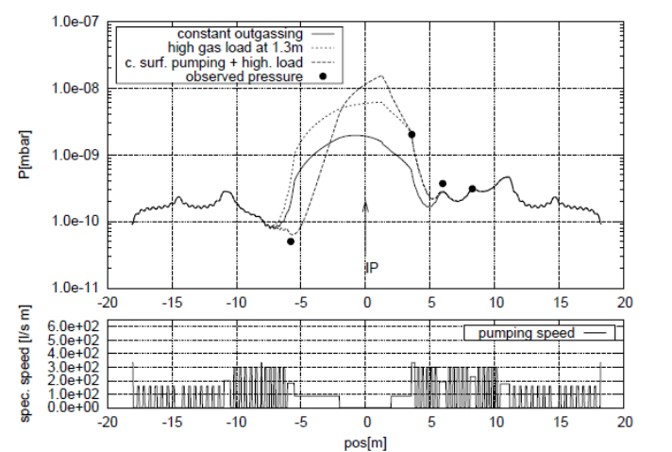
\includegraphics[width=.75	\textwidth]{../../img/hera_badvac_regions.jpg}
	\caption{HERA-II Vacuum pressure distribution around the IP following HERA-II upgrade.  Minima correspond to placement of the vacuum pumps.}
	\label{fig:hera1}
\end{figure}
		
	
\begin{figure}
	\centering
	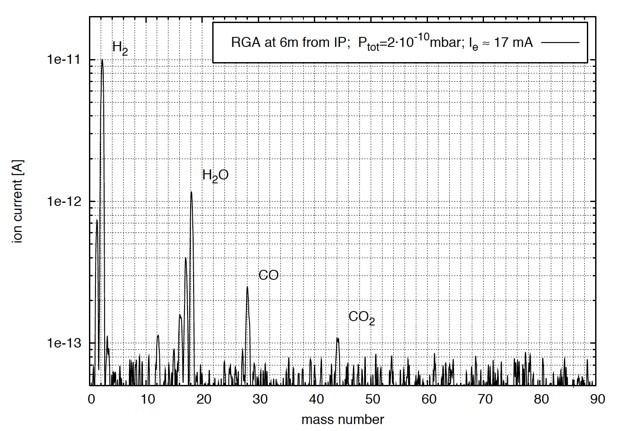
\includegraphics[width=.75\textwidth]{../../img/hera_badvac_comp.jpg}	
	\caption {HERA-II Composition of beampipe gas 6 m from IP. }
	\label{fig:hera2}
\end{figure}
	
\subsection{HERA-II Configuration}
Upstream from the IP, there was a dual layer scintillator detector, referred to as the C5 time-of-flight, which assisted in monitoring the beam-gas background.   Although the rates in the C5 varied as a function of current, they provide a range by which to base the benchmarking study.  Figure \ref{fig:hera3} indicates that the rate in the C5 detector was approximately 10 kHz for I$_{p}$ = 40 mA, for I$_{e+}$ between 2 mA and 7 mA. 

\begin{figure}
	\centering
	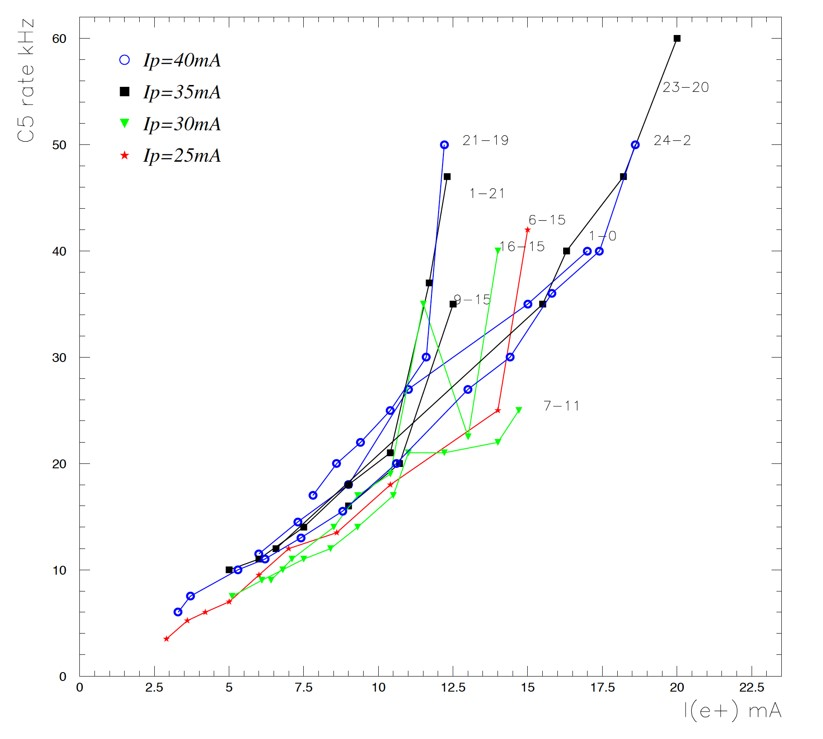
\includegraphics[width=.75\textwidth]{../../img/hera_c5_rate.jpg}
	\caption{C5 rate as a function of HERA \textit{e} beam current for different \textit{p} beam current.  Numeric tags indicate the date and hour of the beginning of \textit{ep} injection for July 2002.}
	\label{fig:hera3}
\end{figure}


\subsection{Approach}

In order to benchmark simulation tools against the observed HERA-II background rates, a virtual detector was modeled after the C5 detector and positioned at the same location relative to the IP.  A beam pipe with the same specifications as the original was filled with a hydrogen target of density proportional to the vacuum quality of the corresponding region at HERA.  The orientation of the C5 detector relative to the IP is shown in Figure \ref{fig:hera4}.  

\begin{figure}
	\centering
	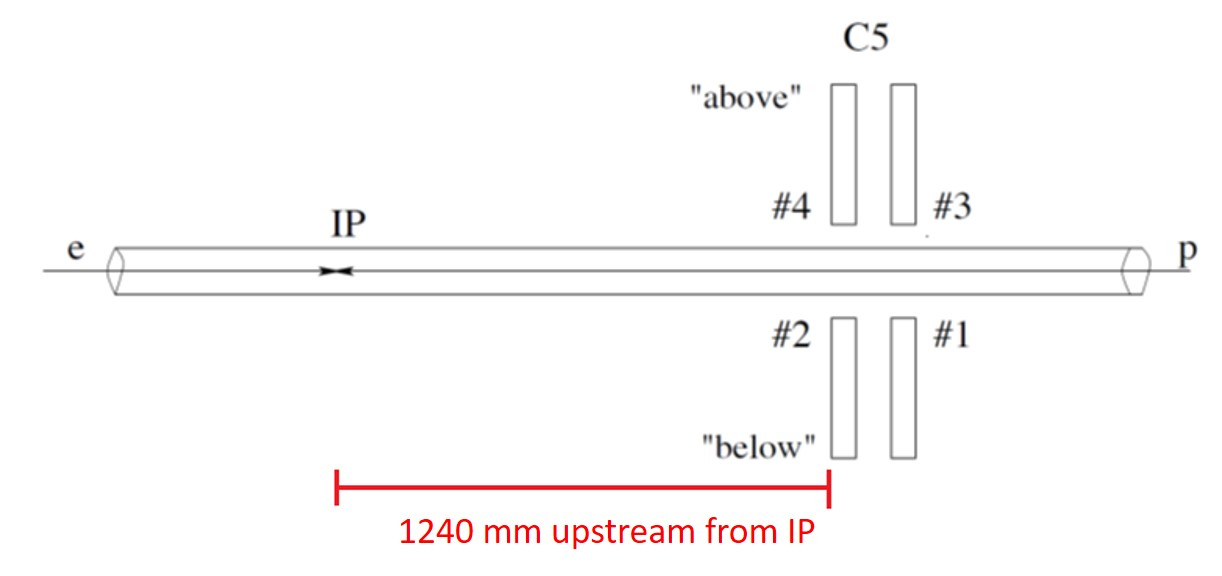
\includegraphics[width=.75\textwidth]{../../img/c5_placement.jpg}
	\caption{C5 detector placement along HERA beamline.}
	\label{fig:hera4}
\end{figure}


Key simulation parameters were either matched to the HERA-II case or scaled.  These are summarized below:


%[beam and beampipeassumptions/parameters] make into a table
\begin{itemize}
	\item HERA-II gate time $\approx$ bunch distance $\approx$ 100ns
	\item Number of proton particles per bunch = $10^{11}$
	\item Proton beam current = 100 mA
\end{itemize}

To replicate the C5 detector, a two-disc scintillator detector was built in GEMC and placed 1240 mm upstream of the IP.  Like the actual C5 detector, the virtual detector was comprised of discs 3 mm thick, separated by 20 mm.  The inner and outer radii also matched the original: $R_{in} = 3.25/2$ cm and $R_{out} = 20.0/2$ cm.  

\begin{figure}
	\centering
	\begin{minipage}{0.45\textwidth}
		\centering
		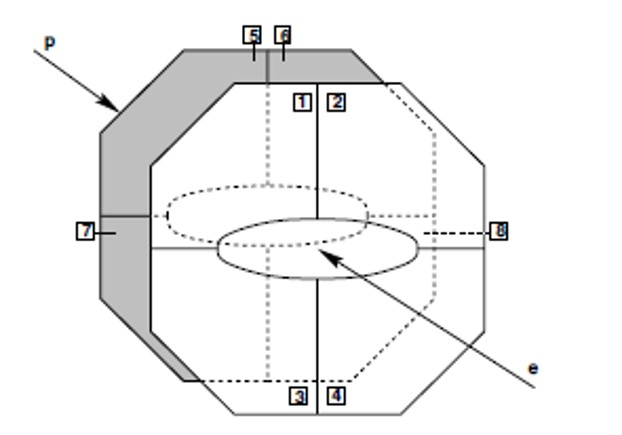
\includegraphics[width=.75\textwidth]{../../img/hera_c5.jpg}
		\caption {Left: Schematic of the actual C5 Time of Flight Detector  }
		
	\end{minipage}\hfill
	\begin{minipage}{0.45\textwidth}
		\centering	\includegraphics[width=.75\textwidth]{../../img/C5_gemc}	
		\caption {Virtual C5 detector rendered in GEMC.}
	\end{minipage}
	
\end{figure}

Likewise, the simple cylindrical beampipe reflected parameters of the original beampipe in HERA-II IP:
%[beam pipe parameters] make into table
\begin{itemize}
	\item material: Al
	\item inner radius: 
	\item thickness: 
	\item Vacuum composition: Hydrogen gas
	\item Vacuum density proportional to $10^{-8}$ mbar $\pm$5 m around IP 
	\item Vacuum density proportional to $10^{-10}$ mbar everywhere else.
\end{itemize}

The internal event generator was positioned directly before the higher pressure region and fired approximately $10^6$ events as a proton beam toward the IP.  All particles hitting the detector, both charged and neutral, were recorded and their information stored in an EVIO file.  Data was analyzed in ROOT after file conversion and making a cut along the $z$ axis in the location of the detector.  The number of neutral particles recorded in the detector was then subtracted from the total, and counts were normalized to $10^6$ events.  This number, along with previously stated assumptions and scale factors, were used to calculate the rate of particles seen in the virtual C5 and compared to HERA-II data.

%insert image of flux in C5 detector for baseline run.
\subsection{Results}
- compare rate: achieved comparable rate in our simulation
show: occupancy plot

\subsubsection{vacuum level dependency}
-varied vacuum level

-rate varied as expected

-plot of dependency

\subsubsection{vacuum length dependency}
-varied vacuum length

-rate varied as expected

-plot of dependency

\subsubsection{physics models}

\subsubsection{beam energy independency}


*validity of simulation
\subsection{Conclusion}







%\begin{figure}
%	\centering
%	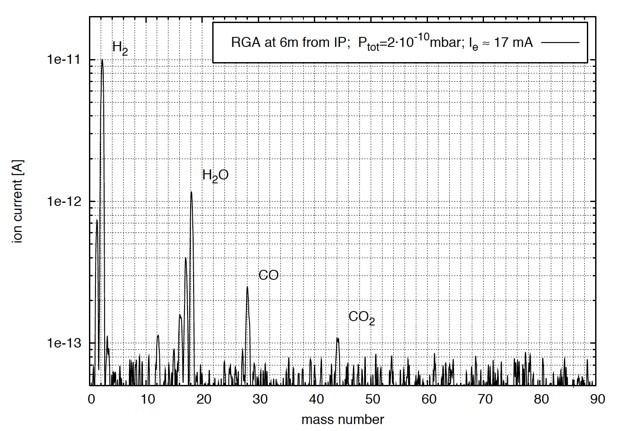
\includegraphics[width=.75\textwidth]{../../img/hera_badvac_comp.jpg}
%	\caption{HERA-II Vacuum pressure distribution in the IR.  The vacuum in the region $\pm$ 5m around the IP deteriorated to $10^{-8}$ mbar, compared to $10^{-10}$ mbar achieved at the pump locations.}
%	\label{fig:hera1}
%\end{figure}

%\begin{figure}
%	\centering
%	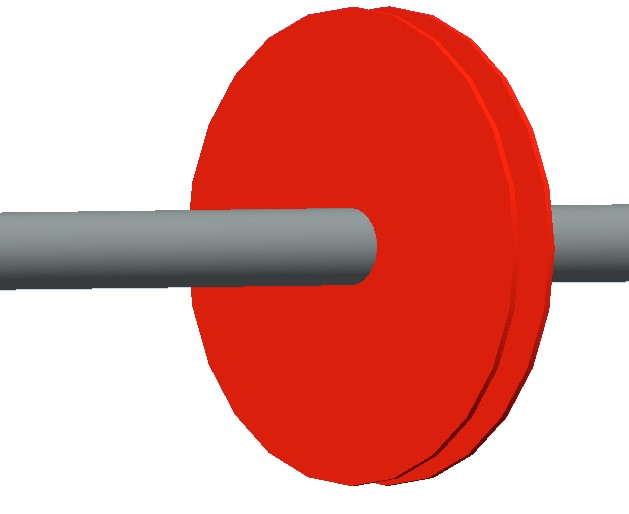
\includegraphics[width=.75\textwidth]{../../img/c5_gemc.jpg}
%	\caption{HERA-II Vacuum pressure distribution in the IR.  The vacuum in the region $\pm$ 5m around the IP deteriorated to $10^{-8}$ mbar, compared to $10^{-10}$ mbar achieved at the pump locations.}
%	\label{fig:hera1}
%\end{figure}

%\begin{figure}
%	\centering
%	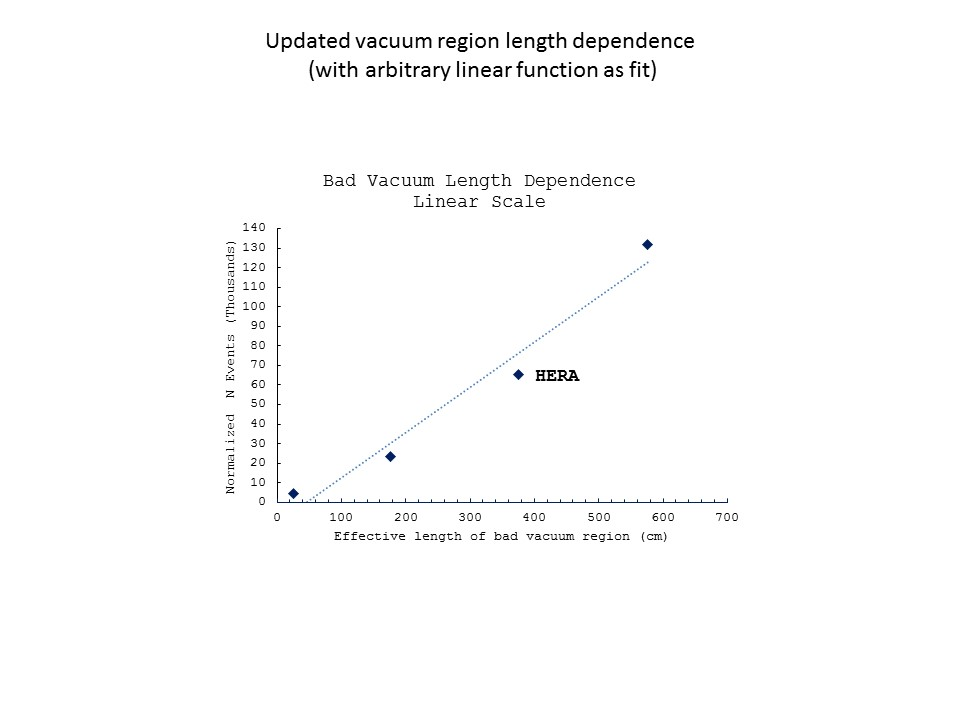
\includegraphics[width=.75\textwidth]{../../img/length_dep_linear.JPG}
%	\caption{HERA-II Vacuum pressure distribution in the IR.  The vacuum in the region $\pm$ 5m around the IP deteriorated to $10^{-8}$ mbar, compared to $10^{-10}$ mbar achieved at the pump locations.}
%	\label{fig:hera1}
%\end{figure}

%\begin{figure}
%	\centering
%	\includegraphics[width=.75\textwidth]{../../img/ length_dep_log.JPG}
%	\caption{HERA-II Vacuum pressure distribution in the IR.  The vacuum in the region $\pm$ 5m around the IP deteriorated to $10^{-8}$ mbar, compared to $10^{-10}$ mbar achieved at the pump locations.}
%	\label{fig:hera1}
%\end{figure}

%\begin{figure}
%	\centering
%	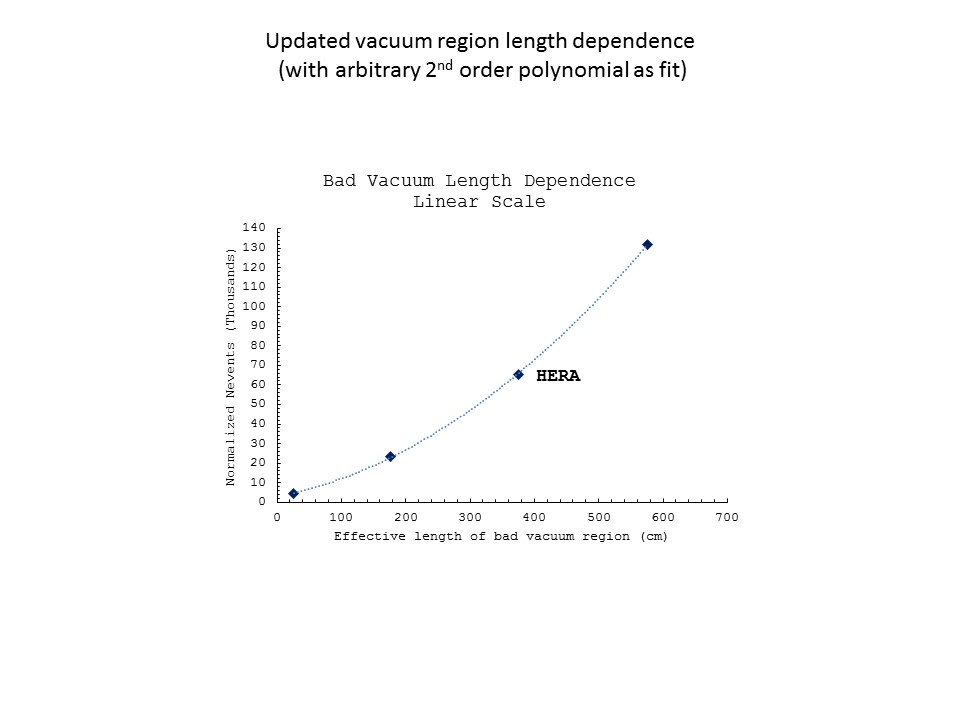
\includegraphics[width=.75\textwidth]{../../img/length_dep_poly.JPG}
%	\caption{HERA-II Vacuum pressure distribution in the IR.  The vacuum in the region $\pm$ 5m around the IP deteriorated to $10^{-8}$ mbar, compared to $10^{-10}$ mbar achieved at the pump locations.}
%	\label{fig:hera1}
%\end{figure}

%\begin{figure}
%	\centering
%	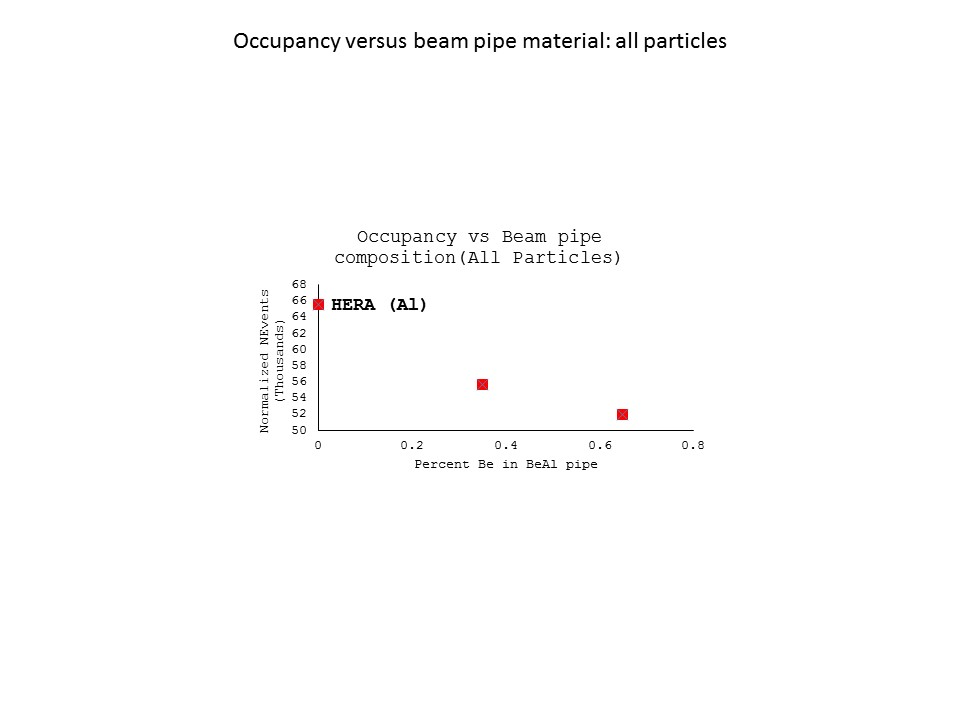
\includegraphics[width=.75\textwidth]{../../img/pipe_comp_all.JPG}
%	\caption{HERA-II Vacuum pressure distribution in the IR.  The vacuum in the region $\pm$ 5m around the IP deteriorated to $10^{-8}$ mbar, compared to $10^{-10}$ mbar achieved at the pump locations.}
%	\label{fig:hera1}
%\end{figure}

%\begin{figure}
%	\centering
%	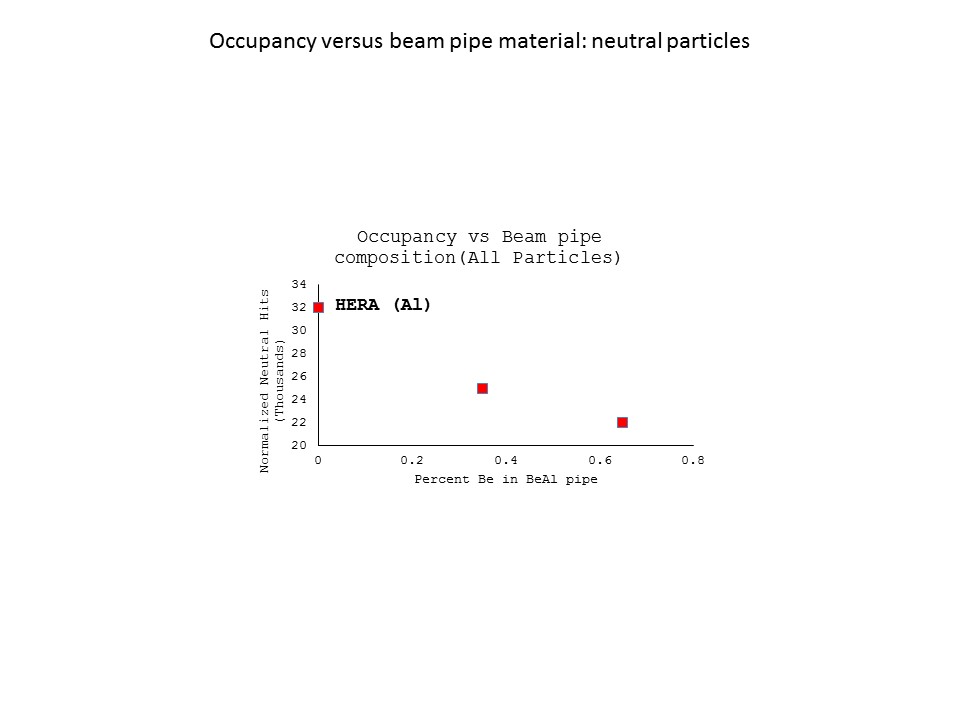
\includegraphics[width=.75\textwidth]{../../img/pipe_comp_neutral.JPG}
%	\caption{HERA-II Vacuum pressure distribution in the IR.  The vacuum in the region $\pm$ 5m around the IP deteriorated to $10^{-8}$ mbar, compared to $10^{-10}$ mbar achieved at the pump locations.}
%	\label{fig:hera1}
%\end{figure}